\section {Математическая модель}
Рассмотрим RQ-систему, на вход которой поступает простейший поток заявок с интенсивностью $\lambda$. Заявка входящего потока, поступая в систему и обнаруживая прибор свободным, занимает его. Прибор, в свою очередь, начинает обслуживание в течение случайного времени, распределенного экспоненциально с параметром $\mu_{1}$. Если же при поступлении в систему заявка обнаруживает прибор занятым, она мгновенно уходит на орбиту и осуществляет там случайную задержу в течение экспоненциально распределенного времени с параметром $\sigma$. В свободное от обслуживания заявок с входящего потока время прибор сам вызывает заявки с интенсивностью $\alpha$ и обслуживает их в течение экспоненциально-распределенного времени с параметром $\mu_{2}$.
\begin{figure}[H]
	\centering
	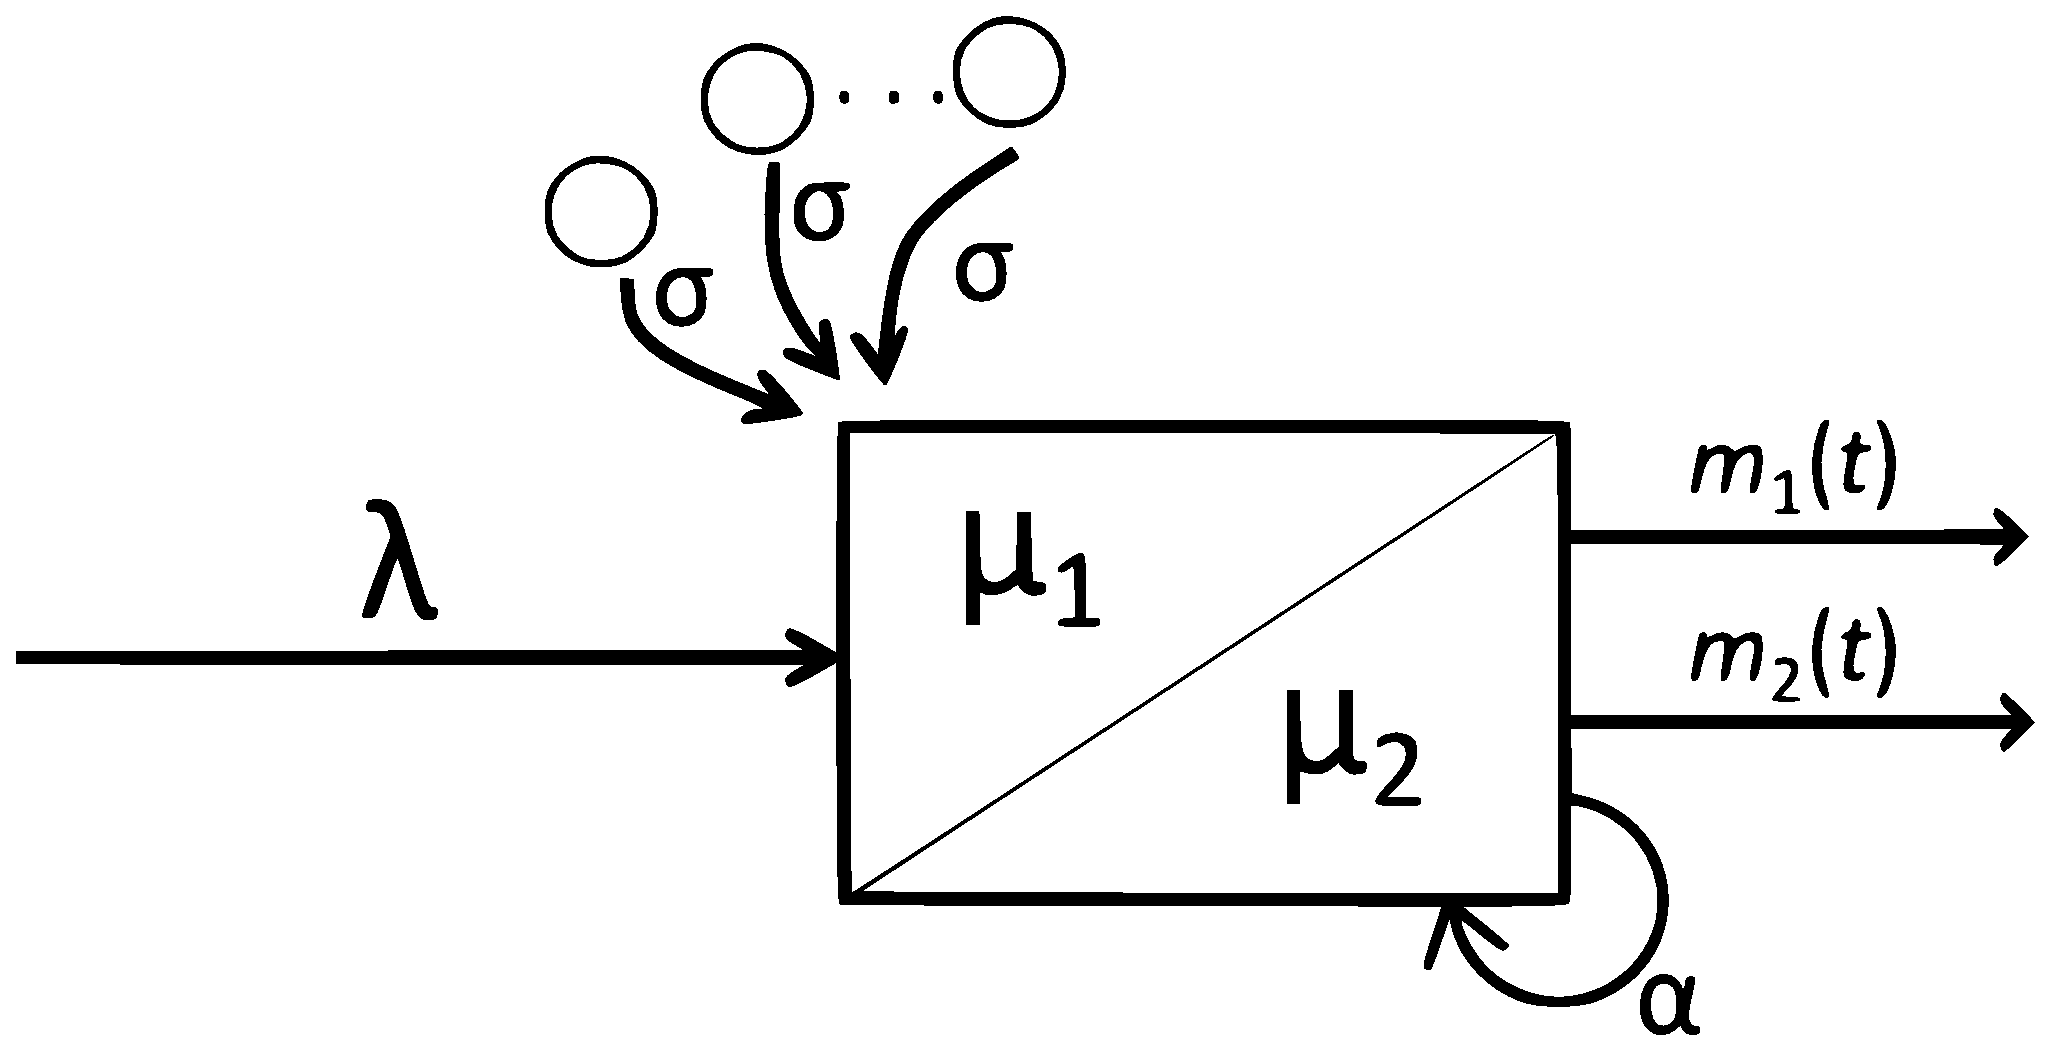
\includegraphics[scale=0.25]{model.eps}
	\caption{Модель системы}
	\label{model_figure}
\end{figure}
Введем следующие обозначения: $\textit{i(t)}$ — число заявок на орбите в момент времени $\textit{t}$, $\textit{k(t)}$ – состояние прибора: $\textit{0}$ – прибор свободен, $\textit{1}$ – прибор занят обслуживанием заявки входящего потока, $\textit{2}$ – прибор занят обслуживанием вызванной заявки; \textit{$m_{1}(t)$} — число обслуженных заявок входящего потока в момент времени $\textit{t}$, \textit{$m_{2}(t)$} — число обслуженных вызванных заявок $\textit{t}$. 
\clearpage